\documentclass[10pt,twocolumn,letterpaper]{article}

\usepackage[margin=40pt]{geometry}
\usepackage{amsmath}
\usepackage{physics}
\usepackage{amssymb}
\usepackage{amsfonts}
\usepackage{hyperref}
\usepackage{thmbox}
\usepackage{geometry}
\usepackage{graphicx}
\usepackage[]{subcaption}
\usepackage[inline]{enumitem}

\newcommand{\R}{\mathbb{R}}
\newcommand{\C}{\mathbb{C}}

\renewcommand{\thefootnote}{\fnsymbol{footnote}}

\author{Haiyang Wang, Nils Jan Fredrik Fryklund, Samuel Potter, Leslie Greengard}
\date{\today}
\title{A Fast Solver for Stokes Flow in 2D: [we need a better title]}

\begin{document}



\maketitle

\begin{abstract}
  In this paper, we exploit the \textit{return to Poiseuille} phenomenon:
  a Stokes flow would quickly develop to the Poiseuille flow along a straight channel.
  This allows us to quickly solve the interior plane Stokes equation
  on a domain that is a union of \textit{standard pieces}.
  Each standard piece is a pipe with inlets/outlets
  being long enough straight channels, 
  such that when two standard pieces are connecting,
  where they connect is in middle of a long
  straight channel\footnote{
    The length of straight channel is greater than 7 times of the width,
    as indicated by Figure~\ref{fig:r2pnumerical}.}, 
  hence the flow at the connection would be close to Poiseuille flow 
  within machine precision.
  Then, instead of solving stokes equation for the global domain,
  we can solve the Stokes equation
  for each standard pieces with boundary condition of Poiseuille velocity profile at inlets/outlets,
  and easily interface these local solutions to build a solution for the global domain.

  Once the Stokes equation with boundary conditions 
  of Poiseuille velocity profile is pre-solved on each standard piece, 
  the standard pieces can be connected to form 
  a complex domain of channel network. 
  Interfacing the solutions of standard pieces would instantly give 
  a high-order accurate solution of Stokes equation for the global domain. 
  For example, in Figure~\ref{fig:connection-error}, 
  interfacing the local solutions took only 0.3 seconds, 
  while directly solving on the global domain took 24 minutes.
\end{abstract}

\begin{figure*}[t]
  \centering
  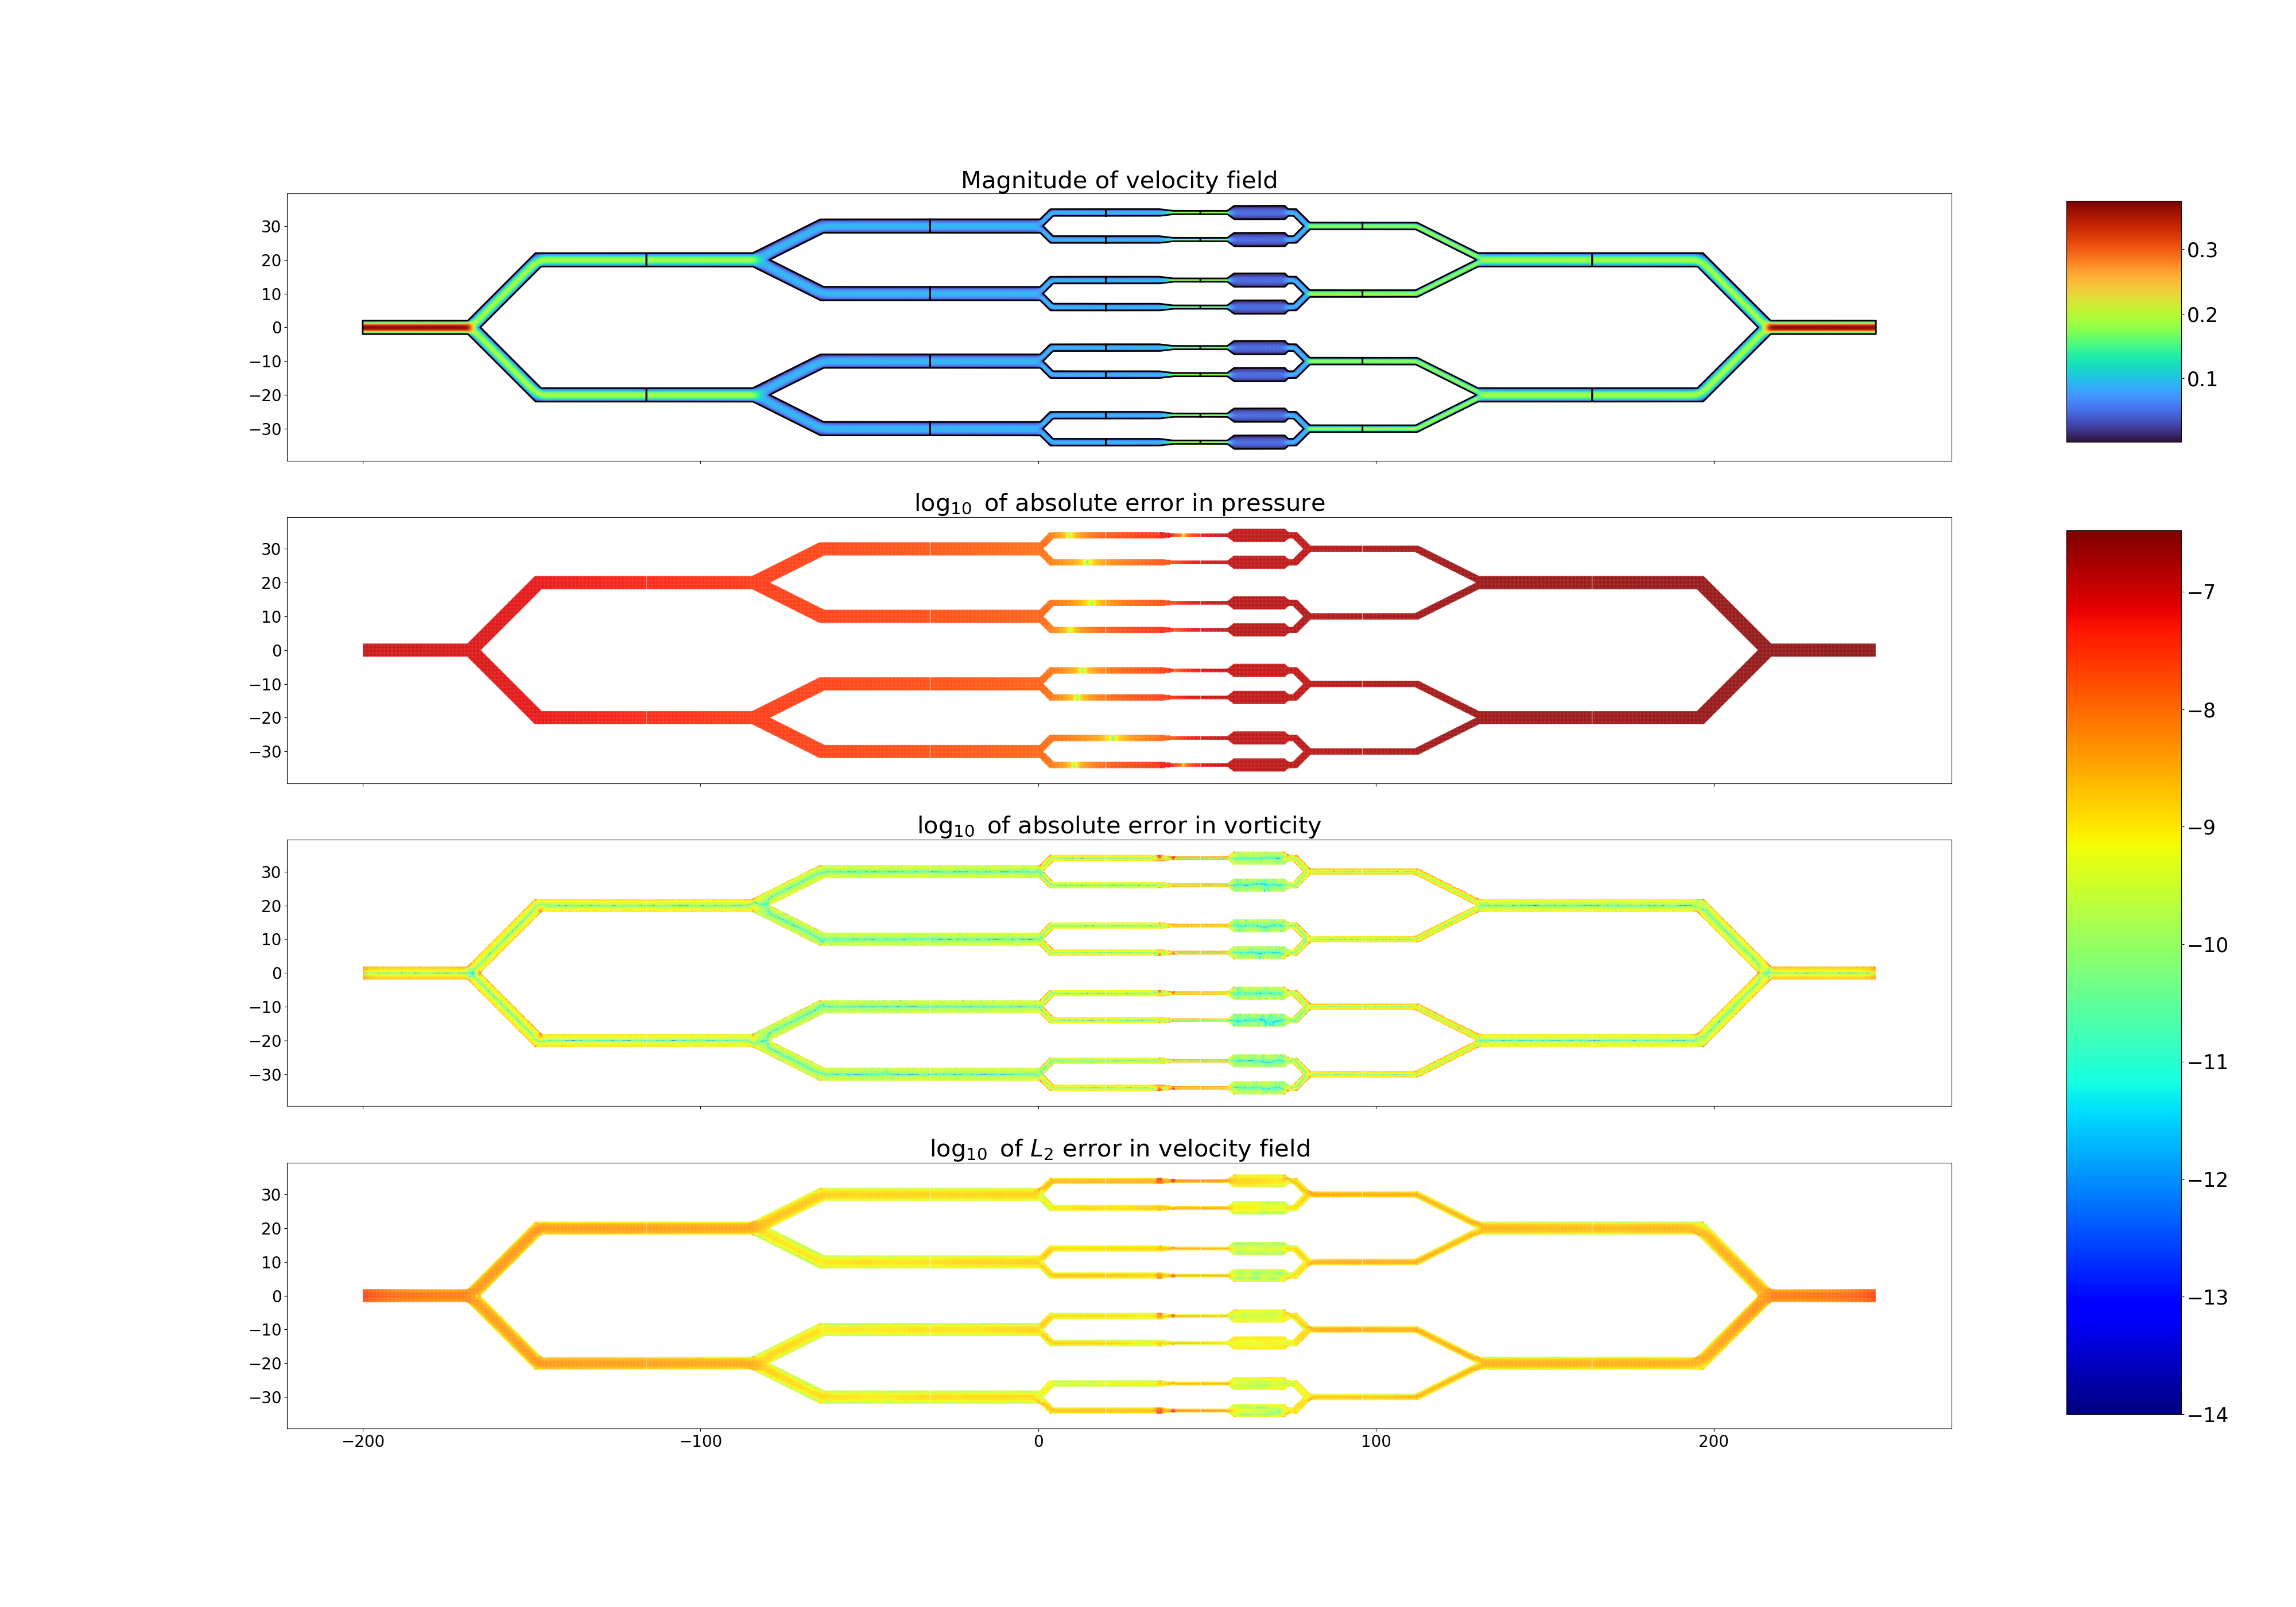
\includegraphics[width=\textwidth]{pic/connection-error-rough.png}
  \caption{
    Solutions of the Stokes equation in a complex channel geometry 
    as a union of 22 pieces of 7 different standard pieces.
    The first sub-figure is a color-plot of magnitude of velocity field 
    inside the domain, 
    with colorbar on its right. 
    The black lines in the first sub-figure marks the boundary of each standard piece.
    The other three sub-figures are color-plots of absolute differences
    between the interfaced solutions and the global solution in pressure,
    vorticity, and velocity field, 
    in the $\log_{10}$ scale, 
    with colorbar on on their right. 
    Each standard pieces are solved with required accuracy of $10^{-12}$ 
    and the global domain is solved with required accuracy of $10^{-10}$.}\label{fig:connection-error}
\end{figure*}

\section{Introduction}

The \textit{return to Poiseuille} phenomenon, 
or \textit{Saint-Venant's principle} in the theory of plane elasticity, 
are well-established from the last century
~\cite{coRecentDevelopmentsConcerning1983,gregoryTractionBoundaryValue1980,horganDECAYESTIMATESBIHARMONIC1989}.
To be more specific, 
in a straight channel with laminar and incompressible incoming flow, 
the flow would quickly converge into a Poiseuille flow: 
the difference of the flow and the Poiseuille flow would 
decay at an exponential rate for Stokes flow. 
Therefore it is a good numerical hypothesis to assume that 
a Stokes flow is Poiseuille in middle of a lone straight channel, 
regardless of the incoming and outgoing flow.

For plane Stokes flow, 
the biharmonic equation formulation have been developed 
within the theory of complex variable from the last century
~\cite{ladyzhenskayaMathematicalTheoryViscous1964}. 
Various numerical methods,
such as boundary integral equation (BIE) and rational function approximation,
have been developed accordingly
~\cite{greengardIntegralEquationMethods1996,trefethenApproximationTheoryApproximation2019}.
In this paper, we use the biharmonic BIE formulation for the plane Stokes
equation from
~\cite{greengardIntegralEquationMethods1996}
to solve the Stokes equation. 


The main idea of this paper is to apply \textit{Return to Poiseuille} as a high
order accurate numerical hypothesis. 
It allows us to pre-solve several standard pieces 
which are pipes with inlets and outlets being long enough straight channels, 
and are with boundary condition of Poiseuille velocity profile. 
Once the standard pieces pre-solved, 
the \textit{Return to Poiseuille} hypothesis allows us to 
interface solutions of Stokes flow on each standard pieces 
to get a solution for  any complex channel networks 
that is a union of the standard pieces. 
Interfacing is by solving a system of linear equations, 
based on the constraints of zero-net-flux and continuity of pressure. 
This system of linear equations can be solved instantly and accurately.

This paper is organized as follows. In Section~\ref{mathprelim}, we define the
Stokes boundary value problem (BVP), the corresponding biharmonic BVP, and then the BIE of it. 
We also mention the analytic evidence and predicted exponential convergence rate for 
the \textit{return to Poiseuille} hypothesis 
in a semi-infinite straight channel. 
Then, we explain how to interface the local solutions of standard pieces 
by a simple example. 
In Section~\ref{sec:numericalmethod}, 
we presents the Nystr\"om discretization of the integral equation, 
which is solved iteratively by Generalized Minimal Residual Method (GMRES).
The numerical experiments of connecting standard pieces and numerical evidence
for \textit{return to Poiseuille} hypothesis are contained in Section~\ref{sec:numericalresults}, 
followed by conclusions and possible further work
in Section~\ref{sec:conclusions}.

\section{Mathematical Preliminaries\label{mathprelim}}

In this section, 
we briefly review the plane Stokes equation, its biharmonic formulation, and the BIE. 
More detailed discussion can be found in~\cite{greengardIntegralEquationMethods1996}. 
Then, we will present an analytic estimate for 
the exponential decay rate of \textit{return to Poiseuille} hypothesis
~\cite{gregoryTractionBoundaryValue1980}, 
and explain how we have applied it as a numerical hypothesis: how to pre-solve each
standard pieces and how to interface the pre-solved solutions for a domain of
connected standard pieces.

\subsection{Boundary Integral Equation}

\paragraph{Stokes Boundary Value Problem.}
Recall that the plane Stokes equation is~\cite{ladyzhenskayaMathematicalTheoryViscous1964}:
\begin{align}
  \nu \Delta u = \frac 1 \rho \pdv{p}{x},\quad & \nu \Delta v = \frac 1\rho \pdv{p}{y}
  \label{stokes}                                                                       \\
  \pdv{u}{x} + \pdv{v}{y}                      & = 0
  \label{continuity}
\end{align}
where $u,v$ are components of velocity, $p$ is the pressure,
$\rho$ and $\nu$ are the density and viscosity.
Another physics quantity, the vorticity, is defined as:
\begin{align}
\zeta  = u_y - v_x
\end{align}

We are interested in interior BVP of Stokes equation
on a bounded $(M+1)$-ply connected domain $D\subset \mathbb R^2$, 
with boundary $\partial D = \Gamma = \Gamma_0 \cup \Gamma_1 \cup \cdots \cup \Gamma_M$, 
where $\Gamma_0$ is the exterior boundary, 
and $\Gamma_1,\ldots, \Gamma_M$ are the interior boundaries. 
This paper concerns with Stokes equation with boundary condition of velocity $u,v$ on the boundary $\Gamma$,
for given functions $h_1,h_2$:
\begin{align}
  u(t) = h_2(t),\quad v(t) = - h_1(t), \quad t\in \Gamma
  \label{bdr-velocity}
\end{align}
% For the specific purpose of this paper,
% the boundary velocity profile is non-slippery,\ i.e. $u=v=0$ everywhere except at the inlets/outlets
% of channels, where a Poiseuille velocity profile is specified.

\paragraph{Biharmonic Equation.} 
$(\ref{continuity})$ implies the existence of the stream function $W(x,y)$ 
such that~\cite{greengardIntegralEquationMethods1996}:
\begin{align}
  \pdv{W}{x} = -v,\quad \pdv{W}{y} = u \label{stream-1}
\end{align}
Following~\eqref{stokes} and~\eqref{continuity}, 
it is easy to see that the stream function 
satisfies the biharmonic equation (\ref{biharmonic}), 
and the Dirichlet BVP ($\ref{bdr-velocity}$) can be rewritten 
as the following biharmonic BVP:
\begin{align}
   & \Delta^2 W(x,y) = \Delta \zeta = 0,                        & (x,y)\in D \label{biharmonic} \\
   & \pdv{W}{x}(t) = h_1(t),\quad \pdv{W}{y}(t) = h_2(t), \quad & t\in \Gamma\label{bih-bv}
\end{align}
% where $h_1,h_2$ are from equation (\ref{bdr-velocity}).

\paragraph{Goursat's Formula.} 
Any plane biharmonic function $W(x,y)$ can be expressed by 
Goursat's formula~\cite{muskhelishviliBasicProblemsMathematical1977}:
\begin{align}
  W(x,y) = \Re (\bar z \phi(z) + \chi (z)) \label{Goursat}
\end{align}
where the Goursat's functions $\phi, \chi$ are analytic functions of complex variable $z = x+yi$.
In the following, we will be identifying $(x,y) \in \mathbb{R}^2$ with $z=x + yi \in \mathbb{C}$.

Velocity, pressure, and vorticity can be conveniently expressed with the Goursat's functions. 
The Muskhelishvili's formula~\eqref{muskhelishvili} expresses velocity field 
and another formula~\eqref{pressure-and-vorticity}
expresses the pressure and vorticity~\cite{muskhelishviliBasicProblemsMathematical1977}:
\begin{align}
  -v + u i & 
    = \pdv{W}{x} + i\pdv{W}{y}
    = \phi(z) + z \overline{\phi'(z)} + \overline{\psi(z)}
    \label{muskhelishvili}\\
  \zeta + \frac{i}{\nu}p & 
    = 4\phi'(z) \label{pressure-and-vorticity}
\end{align} where $\psi = \chi'$.

The biharmonic boundary value problem~\eqref{biharmonic} and ~\eqref{bih-bv}, using
the Muskhelishvili's formula (\ref{muskhelishvili}), can be rewritten as
\begin{align}
  \phi(t) + t\overline{\phi'(t)} + \overline{\psi(t)} = h(t), 
  \quad t \in \Gamma \label{musk-bvp}
\end{align} where $h(t) =  h_1(t) + i h_2(t)$,  
and $t$ is understood as a complex variable.

\paragraph{Sherman-Lauricella Representation.} 
The Sherman-Lauricella representation proposes a specific form of 
the Goursat's functions~\cite{greengardIntegralEquationMethods1996}, 
which can be applied as an ansatz for BIE of the biharmonic BVP~\eqref{musk-bvp} of 
the Stokes equation. 
The Sherman-Lauricella representation is formulated as follows:
\begin{align}
  \phi(z) & =
  \frac {1}{2\pi i} \int_\Gamma \frac{\omega(\xi)}{\xi - z} d\xi
  + \sum_{k=1}^M C_k \log (z-z_k) \label{sl-phi}
  \\
  \psi(z) & =
  \frac {1}{2\pi i} \int_\Gamma \frac{\overline{\omega(\xi)}d\xi +  \omega(\xi)\overline{d\xi}}{\xi - z}
  - \frac {1}{2\pi i} \int_\Gamma \frac{\overline{\xi} \omega(\xi)}{{(\xi - z)}^2} d\xi  \label{sl-psi}
  \\
          & \quad + \sum _{k=1}^M
  \left( \frac{b_k}{z-z_k} + \overline C_k \log (z-z_k) -  C_k \frac{\overline z_k}{z-z_k} \right) \nonumber
\end{align}
where $\omega$ is an unknown complex density on $\Gamma$ to be solved,
$z_k$ are arbitrary prescribed point inside the component curves $\Gamma_k$,
and $C_k, b_k$ are constants defined by:
\begin{align}
  C_k = \int_{\Gamma_k} \omega(\xi) |d\xi|, \quad b_k = 2 \Im\int_{\Gamma_k} \overline{\omega(\xi)} {d\xi}
\end{align}

It is worth-noting that although $\psi, \phi$ might be multiple-valued, 
the velocity, pressure, and vorticity are single-valued functions of $z$.

\paragraph{Boundary Integral Equation.} 
Plugging the Sherman-Lauricella representation
~\eqref{sl-phi} and ~\eqref{sl-psi} into equation (\ref{musk-bvp}), 
and letting a point $z$ in the interior of $D$ approach to 
a point on the boundary $t\in \Gamma$ in~\eqref{musk-bvp}, 
the classical formulae for the limiting values of Cauchy-type integral gives us 
the following boundary integral equation for $\omega$
~\cite{muschelisviliSingularIntegralEquations1972,greengardIntegralEquationMethods1996}:
\begin{align}
  \omega(t)
   & + \frac 1{2\pi i} \int_{\Gamma} \omega(\xi) d\ln \frac{\xi - t}{\overline{\xi - t}} - \frac 1{2\pi i} \int_\Gamma \overline{\omega(\xi)} d \frac{\xi - t}{\overline{\xi - t}} \label{bie} \\
   & + \sum_{k=1}^M \left( \frac{\bar b_k}{\overline{t- z_k}} +  2C_k \log |t-z_k| + \overline{C_k} \frac{t-z_k}{\overline{ t - z_k}} \right) \nonumber                                        \\
   & + \frac{\overline b_0}{\overline{ t - z^*}} \nonumber\\
   & = h(t), 
   \quad\quad\quad\quad\quad\quad\quad\quad\quad\quad\quad\quad t\in \Gamma \nonumber
\end{align}
The extra term $\frac{\overline b_0}{\overline{t - z^*}}$ vanishes 
when the zero-net-flux condition $\Re \int_\Gamma \bar h(t) dt = 0$ is satisfied, 
hence is omitted in the Nystr\"om discretization of~\eqref{bie} later.
The invertibility of this integral equation is similar
to the standard proof of invertibility for elasticity problems
~\cite{muskhelishviliBasicProblemsMathematical1977,greengardIntegralEquationMethods1996}, 
and are omitted. 

\subsection{Return to Poiseuille\label{sec:ret2poi}}

In this section, we will first show the analytic estimate for the
\textit{return to Poiseuille} phenomenon, 
which is based on eigenfunction analysis on a domain of a semi-infinite straight channel 
from the theory of plane elasticity~\cite{gregoryTractionBoundaryValue1980}. 
Then, we explain how to apply the \textit{return to Poiseuille} hypothesis, 
how to build local solutions of each standard pieces, 
and how to interface the solutions on standard pieces. 

\paragraph{Analytic Estimate for Return to Poiseuille. }

On the domain of a semi-infinite straight channel $D_L = \{(x,y)\mid x \ge 0, |y| \le L\}$,
with the boundaries
\begin{align}
  \Gamma_L & = \Gamma_L^1 \cup \Gamma_L^2 \cup \Gamma_L^3                                    \\
           & =\{(0,y)||y| \le L \} \cup \{(x,L)|x\ge 0\} \cup \{(x,-L)\mid x\ge 0\}\nonumber
\end{align}
where $\Gamma_L^2,\Gamma_L^3$ are walls with the non-slippery boundary conditions,
and $\Gamma_L^1$ is the inlet with boundary condition of an
incoming laminar incompressible flow.
\textit{Return to Poiseuille} means that regardless of the boundary velocity profile on $\Gamma_L^1$,
the flow's profile at $x = l$ will converge to Poiseuille flow of same flux as $l\to\infty$.

Without lost of generality, assume there is zero net flux across $\Gamma_L^1$.
Then, \textit{return to Poiseuille} is equivalent to return to the zero flow,
i.e.\ the flows velocity profile at the vertical cross-section $x=l$ would
converge to zero as $l\to\infty$. 
The BVP of this problem can be formulated as the following:
\begin{align}
   & \pdv{W(x,y)}{y}  = W(x,y) = 0,                    & (x,y) & \in \Gamma_L^2 \cup \Gamma_L^3\\
   & \pdv{W(0,y)}{x}  = f(y),\ \pdv{W(0,y)}{y} = g(y), & (0,y) & \in \Gamma_L^1  \label{eq:velocity-condition-at-inlet}
\end{align}
where $f,g$ are continuous and satisfy 
$f(\pm L) = g(\pm L) = \int_{-L}^L g(y)d y = 0$,
for requiring the zero-net-flux and a continuity of boundary condition.

This biharmonic BVP is identical to the self-equilibrated traction BVP in the
theory of elasticity studied ~\cite{gregoryTractionBoundaryValue1980,horganDECAYESTIMATESBIHARMONIC1989,coRecentDevelopmentsConcerning1983}.
According to their result, 
when $f^{\prime\prime\prime},g^{\prime\prime\prime}$ exist and are of bounded variation,
this problem has a unique solution spanned 
by the Papkovich-Fadle eigenfunctions~\cite{gregoryTractionBoundaryValue1980}. 
The absolute value of first eigenfunction is dominated by:
\begin{equation*}
  e^{-x k/2L}, \quad k \simeq 4.2 
  \footnote{$k$ is the smallest positive real parts of the roots of 
the transcendental equation $\sin^2\lambda - \lambda^2=0$.}
\end{equation*}
This gives the decay rate of \textit{return to Poiseuille hypothesis},
which agrees with our numerical experiment in Figure \ref{fig:r2pnumerical}.

\paragraph{Return to Poiseuille as a Numerical Hypothesis.}
Given the analytic estimate above, 
it is easy to see that in a straight channel with length greater than 
8 times of the channel width, 
we can expect the flow to be Poiseuille with 14th digits of accuracy 
at the outlet regardless of the velocity profile on the inlet. 
Therefore, it is appropriate to require the inlets/outlets of 
the standard pieces to be such straight channels, 
and assign the Poiseuille boundary conditions on the inlets/outlets.

% Figure~\ref{fig:connection-error} is a numerical example where the interfaced
% solution is compared with a global solution, and high order accuracy is
% achieved in both pressure, velocity, and vorticity. It is worth-noting that no
% significant numerical error is observed at where the standard pieces are
% connected.

\paragraph{Interface the Solutions on Standard Pieces.}

\begin{figure}[!ht]
  \centering
  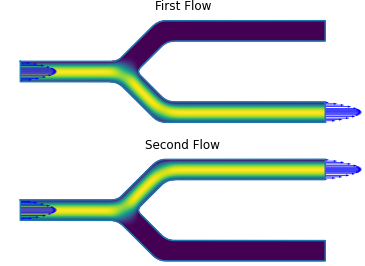
\includegraphics[width=0.4\textwidth]{pic/standard_pipe_flows_demo.png}
  \caption{The 2 generating flows for a Y-shaped standard piece: 
  the color inside the domain denotes the magnitude of the velocity of the flow, 
  the blue arrow denotes the boundary condition of unit-flux Poiseuille velocity profile at the inlets/outlets.}\label{fig:y_2_flows}
\end{figure}

For a standard piece with a total number of $m$ inlets/outlets, 
the boundary conditions of our interest, 
Poiseuille at the inlets/outlets and non-slippery elsewhere, 
can be simply characterized by the flux of the Poiseuille flow at each inlet/outlet. 
The fluxes need to sum to zero, so the boundary conditions is a $m-1$ dimensional space. 
As the Stokes equation is linear, 
this means we only need to solve for $m-1$ flows on the standard piece, 
and superimpose these flows would give us any flow in the standard piece 
with boundary condition of Poiseuille at inlets/outlet and non-slippery elsewhere. 
These flows are called \textit{generating flows} in this paper. 
In practice, for a standard piece, 
we pick one of its inlets/outlets as the inlet for all generating flows, 
each of which would have one of the other inlets/outlets as an outlet. 
Figure~\ref{fig:y_2_flows} shows a standard piece of Y-shaped standard pieces, 
with a total number of 3 inlets/outlets, 
and are pre-solved with 2 generating flows of unit flux. 

With the the generating flows pre-solved for each standard piece, 
interfacing these flows is reduced to finding 
appropriate fluxes of the generating flows of the standard pieces such that:
\begin{enumerate}
  \item The fluxes matches at the interface of connection\label{cond:flux-match}.
  \item The pressure is a continuous function across the global  domain.\label{cond:pressure}
\end{enumerate}
The second condition is needed only when the global domain is not simply connected. 

To demonstrate how these two conditions are turned into 
a linear system of equations for interfacing local solutions, 
let us consider the specific example in Figure~\ref{fig:interface_problem_0}, where the global domain 
is two connected Y-shaped standard pieces. 
The global domain is given with flux $f_{-1} = 1$ (incoming) at the left inlet 
and flux $f_{-2}=1$ (outgoing) at the right outlet. 
Each standard piece has two fluxes of generating flows need to be solved for, 
so there are total number of $4$ fluxes $f_0,f_1,f_2,f_3$ needs to be solved for. 

This problem can be abstracted into a problem 
on a directed graph as in Figure~\ref{fig:interface_problem_1},
where the the nodes $V_0,V_1,V_2,V_3$ denotes the interfaces among the standard pieces 
and global boundary conditions of fluxes, 
The edge $E_{0,1},E_{0,2},E_{31},E_{32}$ represents the generating flows 
with the fluxes $f_0,f_1,f_2,f_3$ to be solved for. 
The fluxes $f_{-1},f_{-2}$ are given on superficial edges representing the boundary fluxes of the global domain.

\begin{figure}[!ht]
  \centering
  \begin{subfigure}[b]{0.45\textwidth}
    \centering
    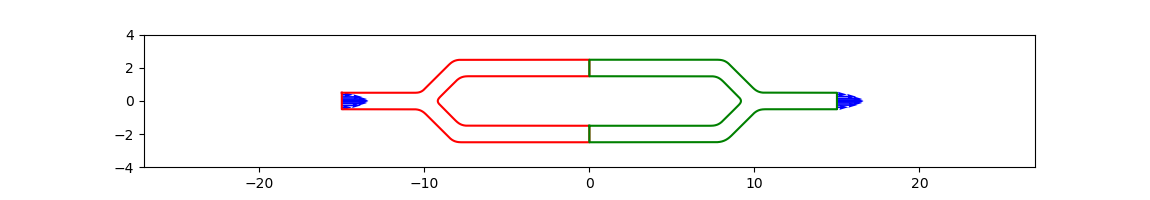
\includegraphics[width=\textwidth]{pic/simple-interface-problem.png}
    \caption{The interface problem}\label{fig:interface_problem_0}
  \end{subfigure}
  \begin{subfigure}[b]{0.45\textwidth}
    \centering
    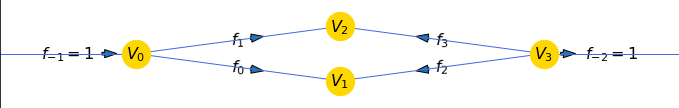
\includegraphics[width=\textwidth]{pic/simple-interface-problem-network.png}
    \caption{The directed graph for the interface problem}\label{fig:interface_problem_1}
  \end{subfigure}
  \caption{A simple interface problem with 2 Y-shaped standard pieces.}\label{fig:simple-interface-problem}
\end{figure}

The interface condition~\ref{cond:flux-match} of agreeing fluxes at the interfaces, 
in the directed graph, 
can be understood as the following: 
at each node, the incoming fluxes should be equal to outgoing fluxes. 
Requiring this to be true at all nodes gives us
the following linear system of equations:
\begin{align}
  \begin{pmatrix}
    1 & 1 & 0 & 0\\
    1 & 0 & 1 & 0\\
    0 & 1 & 0 & 1\\
    0 & 0 & 1 & 1\\
  \end{pmatrix}
  \begin{pmatrix}
    f_0\\
    f_1\\
    f_2\\
    f_3\\
  \end{pmatrix}
  =
  \begin{pmatrix}
    f_{-1}\\
    0\\
    0\\
    -f_{-2}\\
  \end{pmatrix}
  =
  \begin{pmatrix}
    1\\
    0\\
    0\\
    -1\\
  \end{pmatrix} \label{eq:interface-flux-match}
\end{align}
This matrix has rank 1 deficiency. 
This is due to the 1 cycle in the graph, 
and can be resolved by adding the continuity of pressure condition~\ref{cond:pressure}. 

Continuity of pressure, or single-valued-ness of pressure, 
can be interpreted as that the pressure $p_i$ at each node $V_i$ is 
a well-defined single-valued function.
And on a cycle, this means that 
the pressure drops along the cycle would sum to zero. Therefore, we can gain a new equation: 
\begin{align}
  p_{10} + p_{31} + p_{23} + p_{02} =0 \label{eq:pressure-cycle}
\end{align}
where $p_{ij}$ is the pressure drop from node $V_j$ to node $V_i$. 
The pressure drops $p_{ij}$ depends linearly on the fluxes of generating flows of the standard pieces, 
For this case, $p_{10}, p_{02}$ are linear functions of $f_0,f_1$, 
and $p_{31}, p_{23}$ are linear functions of $f_2,f_3$. 
These linear functions can be computed in the pre-solving process,
and for this example, they are
\begin{align}
  \begin{pmatrix} p_{10} \\ p_{02} \end{pmatrix} 
  &= \begin{pmatrix}
    46.02 & 14.78 \\
    -14.78 & -46.02
  \end{pmatrix}
  \begin{pmatrix}
    f_0\\
    f_1
  \end{pmatrix} \label{eq:pd1} \\
  \begin{pmatrix} p_{31} \\ p_{23} \end{pmatrix} 
  &= \begin{pmatrix}
    -46.02 & -14.78 \\
    14.78 & 46.02
  \end{pmatrix}
  \begin{pmatrix}
    f_2\\
    f_3
  \end{pmatrix}\label{eq:pd2}
\end{align}

Combining equations~(\ref{eq:pressure-cycle}),~(\ref{eq:pd1}) and~(\ref{eq:pd2}), we have:
\begin{align}
  (46.02-14.78)(f_0 - f_1 - f_2 + f_3) = 0
\end{align}
which completes~\eqref{eq:interface-flux-match} to a full rank linear system of equations 
and with the solutions $(f_0,f_1,f_2,f_3) = (0.5,0.5,-0.5,-0.5)$. 

The process of interfacing local solutions in the example of Figure~\ref{fig:simple-interface-problem} 
can be generalized into a algorithm for interfacing of any connected standard pieces. 
The key idea of the algorithm is rather simple: 
generating the appropriate linear equations of matching fluxes and matching pressure drops,  
and then solving for fluxes of generating flows.
However, it involves troublesome bookkeeping of the correspondence between the directed graph 
and the generating fluxes and pressure-drops of each standard pieces, 
so the complete description of the algorithm is omitted. 
\footnote{One can find source code for this algorithm at  \href{https://github.com/WangHaiYang874/stokes2d/blob/main/src/pipe_system/pipe_system.py}{github.com/WangHaiYang874/stokes2d}}

% \paragraph{Numerical Stability of Interface Algorithm}
% The numerical stability of the connecting algorithm can be analyzed as follows. 
% The condition of matching fluxed~\ref{cond:flux-match} is translated to the linear equation~\eqref{eq:interface-flux-match},
% which contains only $1,0$ and therefore no inaccuracy is introduced. 
% The only inaccuracy is introduced by computing of the matrices in~\eqref{eq:pd1} and~\eqref{eq:pd2} in the pre-solving process. 
% Each entries of the matrices of pressure drops can be computed with required accuracy of $\epsilon=10^{-12}$, Therefore ... 

\section{Description of Numerical Methods\label{sec:numericalmethod}}

In this section,
we will first present Nystr\"om discretization of BIE (\ref{bie}).
And we will briefly mention several other numerical techniques we have adopted that
are established for solving such BIE. 

\subsection{Boundary Integral Equation}

The boundary curve $\Gamma_k$ is given by the parametrization $\Gamma_k = \{
  t^k(a): a\in \left[A_k,A_{k+1}\right]\}$, 
  and discretized into $N_k$ points $t^k_i = t^k(a^k_i)$.
The exterior boundary $\Gamma_0$ is parameterized in the counter-clockwise orientation, while the interior boundaries
are parameterized in the clockwise orientation.
Associate to each point $t^k_j$ are the unknown complex density $\omega^k_j$, 
  the derivative $d^k_j = t^{k\prime}(a^k_j)$, 
  and the quadrature weight $w^k_j$. 
In total, we have $N= \sum_{k=0}^M N_k$ points. 
The Nystr\"om discretization of BIE (\ref{bie}) is:
\begin{align}
  \omega_j^k
  + \sum_{m=0}^{M}\sum_{n=1}^{N_k} K_1(t^k_j,t^m_n) \omega^k_j
  + \sum_{m=0}^{M}\sum_{n=1}^{N_k} K_2(t^k_j,t^m_n) \overline{\omega^k_j} = h^k_j
  \label{nystrom}
\end{align} where $h^k_j = h(t^k_j)$ and the kernels $K_1, K_2$ are given by
\begin{align}
  K_1(t^k_j, t^m_n)
   & = \frac{w^m_n}{\pi} \Im (\frac{d^m_n}{t^m_n-t^k_j}) + K_1^s(t^k_j,t^m_n)\\
  K_2(t^k_j, t^m_n)
   & = \frac{w^m_n}{\pi} \frac{\Im((t^m_n-t^k_j)\overline{d^m_n})}{(\overline{t^m_n - t^k_j)^2}}  + K_2^s(t^k_j,t^m_n)\\
  K_1^s(t^k_j,t^m_n) 
    & = \delta_m w^m_n \left(\frac{i\overline{d^m_n}}{\overline{t^k_j - z_m}}
    + 2 \log |t^k_j - z_m| \right)\\
  K_2^s(t^k_j,t^m_n) 
    & = \delta_{m}w^m_n \frac{t^k_j-z_m-id^m_n}{\overline{t^k_j - z_m}}
\end{align}
where $\delta_m = 1$ excepts for $\delta_0 = 0$. 

In the limiting case of $t^k_j = t^m_n$, the values of $K_1,K_2$ are:
\begin{align}
  K_1(t^k_j, t^k_j) 
    & = \frac{w^k_j \kappa^k_j|d^k_j|}{2\pi} + K_1^s(t^k_j,t^k_j)\\
  K_2(t^k_j, t^k_j) 
    & = -\frac{w^k_j\kappa^k_j(d^k_j)^2}{2\pi|d^k_j|} + K_2^s(t^k_j,t^k_j)
\end{align}where $\kappa^k_j$ is the signed curvature at the point $t^k_j$.

By separating the real and imaginary parts of The Nystr\"om discretizetion \eqref{nystrom}, we can get a $2N\times 2N$ matrix equation:
\begin{align}
  \begin{pmatrix}
    I + \Re(K_1 + K_2) & \Im(-K_1 + K_2) \\
    \Im(K_1 + K_2) & I + \Re{K_1 - K_2}  
  \end{pmatrix}
  \begin{pmatrix}
    \Re \omega  \\ \Im \omega 
  \end{pmatrix}
  =
  \begin{pmatrix}
    \Re h \\ \Im h
  \end{pmatrix}
  \label{nys-mateq}
\end{align}
This equation is solved iteratively by the GMRES \cite{saadGMRESGeneralizedMinimal1986}.
For each GMRES iteration, evaluating the left hand side of \eqref{nys-mateq}
is done by a biharmonic fast multipole method (FMM) 
provided by the Flatiron Institute \cite{FlatironinstituteFmm2d2022}, 
which reduce the time complexity of each GMRES iteration from $O(N^2)$ to $O(N)$, 
and the overall space complexity from $O(N^2)$ to $O(N)$. 

The matrix equation \eqref{nys-mateq} has rank-1 deficiency, 
due to the zero-net-flux condition $\Re \int_\Gamma \overline{h(t)} dt = 0$ 
of Stokes equation. This rank-1 deficiency can cause GMRES to converge slowly. 
By adding a double layer term into \eqref{nys-mateq} would fill up 
the nullspace of this BIE and avoid GMRES stagnating \cite{zhangFastDirectSolver2022}. 

Once $\omega$ is solved, 
\eqref{muskhelishvili}, \eqref{pressure-and-vorticity}, \eqref{sl-phi}, and \eqref{sl-psi}, 
can be applied to evaluate the velocity, pressure, and vorticity inside the domain. 
However, near the boundary, these evaluation involves nearly singular integrals. 
Thus, we have adopted the methods from
~\cite{wuSolutionStokesFlow2020,helsingEvaluationLayerPotentials2008} 
for accurate evaluation of these physics quantities near the boundary.

\subsection{Discretization and Smoothness of the Boundary}

The boundary curves is discretized into a set of Gauss-Legendre panels, 
with certain heuristics applied to ensure that each panel resolves 
the curve accurately enough. 
Moreover, if two non-neighboring panels are very close to each other, 
the evaluation of left hand side of \eqref{nys-mateq} might contain 
nearly singular integrals. Hence, such panels are further refined. 
These discretization strategies are nothing new from
the detailed description of an adaptive refinement discretization scheme 
in~\cite{wuSolutionStokesFlow2020}.  

The key to spectral convergence of GMRES is to have smooth boundary. 
For piecewise smooth boundary, 
a graded meshes can also be used to resolve corner singularity
~\cite{wuSolutionStokesFlow2020}. 
Here in this paper, we have used purely smooth boundary curves, 
and it is explained as follows.

At each of the inlets and outlets, there are two right angle corners. 
These two right angles are avoided by adding superficial cap at the inlet and outlet, 
and putting the Poiseuille boundary conditions on the superficial cap instead. 
Figure~\ref{fig:superficial-cap} demonstrates an example, 
where the orange line demonstrate the original cornered geometry with Poiseuille boundary
conditions, and the blue dashed-line denotes the superficial caps, 
with the same Poiseuille boundary condition denoted by the dark-blue color. 
The standard pieces are still connected along the orange straight line, 
in which case the blue caps are still in middle of a long straight channel. 
Therefore, the \textit{return to Poiseuille} hypothesis still holds at the 
blue caps and it is numerically stable to 
transfer the Poiseuille velocity profile from the orange lines 
to the blue caps. 
These caps are smooth curves constructed as in Appendix B. of
~\cite{baggeHighlyAccurateSpecial2021}. 

Other corners of the geometry are smoothed as in Figure~\ref{fig:smooth-corner}. 
This is achieved by a convolution the coordinates of the corner 
with a smooth bump function \cite{epsteinSmoothedCornersScattered2016}.

\begin{figure}[!ht]
  \centering
  \begin{subfigure}[b]{0.4\textwidth}
    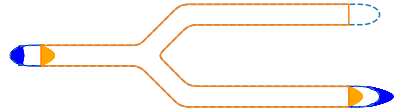
\includegraphics[width=\textwidth]{pic/superficial_cap_demo.png}  
    \caption{Superficial Cap}\label{fig:superficial-cap}
  \end{subfigure}
  \begin{subfigure}[b]{0.4\textwidth}
    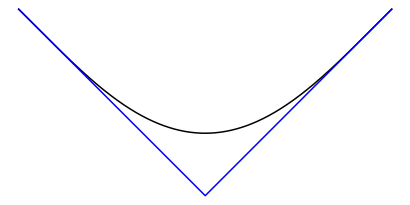
\includegraphics[width=0.8\textwidth]{pic/smoothed_corner.png}
    \caption{A Smoothed Corner}\label{fig:smooth-corner}
  \end{subfigure}
  \caption{Smoothed Geometry}
\end{figure}

\section{Numerical Results and Discussion\label{sec:numericalresults}}
\begin{figure}[!ht]
  \centering
  \begin{subfigure}[b]{0.4\textwidth}
    \centering
    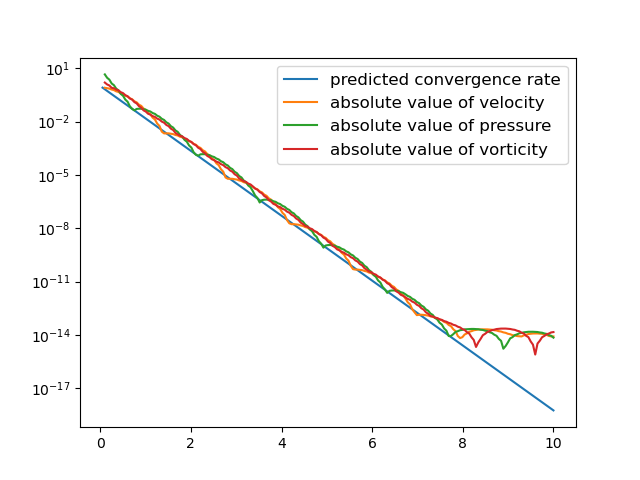
\includegraphics[width=\textwidth]{pic/rtp_cv.png}
    \caption{Numerical Convergence rate of return to Poiseuille flow in a straight channel}
    \label{fig:rtp_cv}
  \end{subfigure}
  \begin{subfigure}[b]{0.4\textwidth}
    \centering
    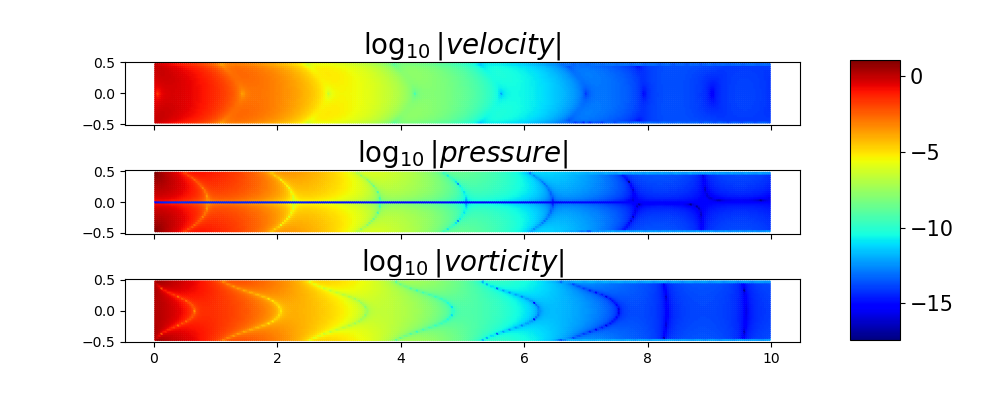
\includegraphics[width=\textwidth]{pic/rtppipe.png}
    \caption{$\log_{10}$ of the absolute value of the velocity, vorticity, and pressure within the straight channel.}
    \label{fig:rtppipe}
  \end{subfigure}
  \caption{Numerical exponential rate for return to Poiseuille flow.
    This is solution of Stokes BVP on a straight channel of length 10 and width 1,
    with non-slippery boundary condition on the top and bottom walls,
    an incoming flow (smooth and randomly generated) of zero-net-flux on the left inlet,
    and no outgoing flow on the right outlet.
    (a) The semilogy of magnitude of velocity, pressure, and vorticity
    along each vertical cross section along the channel.
    (b) The color plot of the magnitude of velocity, pressure, and vorticity in $\log_{10}$ scale in the straight channel.
  }
  \label{fig:r2pnumerical}
\end{figure}

\subsection{Numerical Evidence of Return to Poiseuille}
The numerical evidence for return to Poiseuille phenomenon is 
demonstrated on a straight channel of width $1$ 
and length $8$ as in Figure \ref{fig:r2pnumerical}.
On the left boundary, a smooth velocity profile is imposed. 
This velocity profile is an arbitrarily picked smooth function 
that satisfies the requirement of equation (\ref{eq:velocity-condition-at-inlet}). 
On the rest of the curve, non-slippery condition is imposed.

Figure \ref{fig:rtp_cv} shows that the rate of 
returning to the zero flow is agreed with the predicted rate 
from Section \ref{sec:ret2poi} up to 14th digits of accuracy. 
Figure \ref{fig:rtppipe} is a color plot where the color indicates
the $\log_{10}$ of absolute value of the velocity, pressure, and vorticity. 
All of them decay to zero at the same exponential rate. 

\subsection{A More Complicated Example}
Figure~\ref{fig:connection-error} is an example of 22 pieces of
7 different kinds of standard pieces. 
Each of the standard pieces are solved with 12 digits of accuracy,
and are compared with a solution on the global geometry with 10 digits of accuracy. 

No major numerical error can be observed near the interface of two standard pieces. 
This could mean that the \textit{return to Poiseuille} is indeed good numerical hypothesis. 

% Should I include a detailed analysis of the interfacing algorithm here? 
% In short, suppose we can evaluate pressure with accuracy $\epsilon$, 
% then the relative error of fluxes of the generating flows are bounded by m^2\epsilon.
% where m is the total number of generating flows. Better, m^2 can be replaced by the
% number of entries in the matrix generated by interfacing algorithm. 


\section{Conclusions\label{sec:conclusions}}

We have presented an usage of the \textit{return to Poiseuille} phenomenon
that turns the problem of solving Stokes flow on a geometry generated by 
several standard pieces into solving for weights on edges of a directed graph. 
It provides a way to instantly get high order accurate solutions for 
the special geometries considered in this paper. 

One nature extension of this work is to make a 3D version, 
where more interesting standard pieces can be included.
The major weakness of this work is that the current scheme relies heavily 
on the return to Poiseuille hypothesis, therefore it is cannot
include particles in the flow: 
if we have a particle near the interfaces, the interface cannot have
boundary conditions of a Poiseuille flow. 
In this regard, a more useful extension of this work is to be able to add particles in the fluid simulations. 
This interface idea can be extended to not only interface pre-solved Poiseuille flows, 
but also a much larger class of pre-solved characteristic flows. 
And the influence of particles can be coupled with fast direct solvers.
Therefore enabling fast and accurate simulations of Stokes flow with particles in it. 
% The latter part of last paragraph is what I remembered from a conversation with professor Greengard, 
% and I am sure I don't understand how this would really work out. 
% I am not sure if I should include this part. 

\section*{Acknowledgements\label{sec:acknowledgements}}

We thank Manas Rachh and Charles Peskin for many useful discussions pretaining to this work. 
We thank Manas Rachh and Libin Lu for providing support for the Flatiron Institute's FMM2D library \cite{FlatironinstituteFmm2d2022}.

\bibliographystyle{plain}
\bibliography{references}
\end{document}